\chapter{Ejercicio de seguimiento autónomo de carreteras con un  dron}\label{cap.followroad}
En este capítulo se va a describir la segunda práctica actualizada para el elenco de ejercicios de robótica de \textit{Robotics-Academy}. Esta práctica se llama \textit{Follow Road} y se explicar todo lo relacionado con su infraestructura, las dos plantillas \textit{software} (nodos ROS y cuadernillos \textit{Jupyter}), la solución desarrollada y su validación experimental.

\section{Enunciado}\label{sec.enunciado}
Para el estudiante, el objetivo de esta práctica, es el desarrollo de un algoritmo que dote de la inteligencia necesaria a un dron para que sea capaz de seguir una carretera. En este caso, se deben controlar la altitud, la velocidad y el giro del dron para realizar un correcto seguimiento de la carretera. Esto supone un desafío para el alumno que deberá tener un control absoluto del robot en todo momento.

Para desarrollar la solución de esta práctica, el alumno debe enfrentarse a diversos problemas relacionados con la robótica. El primero de ellos es la visión, el alumno deberá realizar un procesado de imagen para filtrar los objetos que le interesen. En este caso deberá filtrar la carretera. El segundo problema a abordar es el control de movimiento del dron. En este caso debe ser muy preciso porque se manejan alturas, además de giros y velocidades.

El desafío de esta práctica reside en la dificultad de mantener el dron estable en todo momento y adecuar sus movimientos al procesado de imagen que se realice. Esto supone solucionar los problemas anteriores de manera conjunta. Además, es necesario el desarrollo de un algoritmo robusto para evitar que el dron se estrelle o tenga un comportamiento anormal en casos extremos o en situaciones no previstas.

\section{Infraestructura}
Este ejercicio funciona en un determinado escenario de \textit{Gazebo}, que ha habido que desarrollar y con un dron importado que ha tenido que ser modificado. El dron tiene dos cámaras y un controlador de velocidad y altitud que proporciona movimiento (Figura \ref{fig.infraestructura_fr}).

\begin{figure}[H]
  \begin{center}
    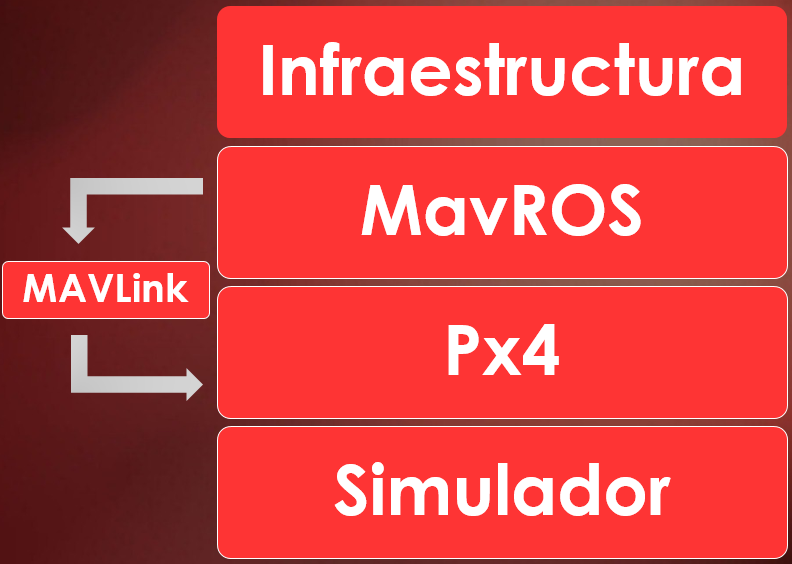
\includegraphics[width=0.4\linewidth, height=8cm]{figures/infraestructura_fr.png}
		\caption{Infraestructura del ejercicio Follow Road}
		\label{fig.infraestructura_fr}
		\end{center}
\end{figure}

\subsection{Modelo del dron en Gazebo}
Para la realización de esta práctica se ha escogido el modelo ``Iris'' de dron. Este modelo consta de un cuerpo principal, en el que va instalado el \textit{hardware}, cuatro rotores, una antena y dos cámaras. La inteligencia del dron, tanto real como simulado, viene dada por el sistema de pilotaje automático \textit{Px4}.

\begin{figure}[H]
	\begin{center}
	    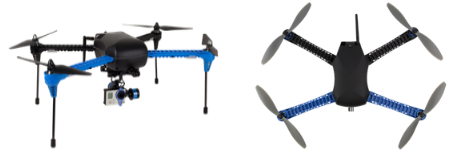
\includegraphics[width=0.98\textwidth]{figures/iris.png}
		\caption{Ilustraciones del dron ``Iris''}
		\label{fig.iris}
	\end{center}
\end{figure}

\subsubsection{Cámara}
La cámara proporciona al dron visión del escenario en el que se encuentra. En esta práctica son necesarias dos cámaras, una frontal y otra ventral, para tener una visión del entorno tanto en la parte delantera del dron, para evitar obstáculos, como inferior para observar correctamente la carretera.

El \textit{plugin} de la cámara en Gazebo es proporcionado por \textit{ROS}. Este \textit{plugin} proporciona el código necesario para conectar una cámara con una velocidad de refresco de 30 imágenes por segundo con una longitud focal de 277 milímetros. El tamaño de las imágenes, obtenidas periódicamente, es de 360x240 píxeles y están en formato crudo RGB. Con estas características, el dron puede recoger imágenes a una velocidad lo suficientemente rápida y a una distancia apropiada, para procesar las imágenes y evitar los obstáculos con suficiente antelación.

\subsubsection{Sensor de posición}
Con este sensor, el dron es capaz de conocer su posición 3D en el mundo. Este sistema se implementa gracias al GPS que incorpora el dron y le permite conocer su latitud y longitud en el escenario en el que se encuentre. \textit{MavROS} incorpora \textit{topics} para conocer esta posición. El \textit{topic} utilizado ofrece la posición del dron en coordenadas relativas al lugar de despegue del dron. Esta funcionalidad viene soportada en el \textit{plugin setpoint\_position}.

\subsubsection{Rotores}
El dron está formado por cuatro rotores que permiten su movimiento. Para el control de estos rotores, se incorpora un \textit{plugin} de control de rotor por cada uno de los rotores del dron. Este \textit{plugin} es proporcionado por \textit{Px4}. Dentro de \textit{MavROS} se usa el \textit{plugin} \textit{setpoint\_raw} para mover el dron, al que se accede con el \textit{topic /mavros/setpoint\_raw/local}. 

\subsection{Escenario de Gazebo}
Para esta práctica se ha actualizado el escenario inicial del que disponía la práctica y se han arreglado problemas que presentaba relacionados con la visualización del suelo, un nuevo modelo de casa y la incorporación del modelo del dron nuevo. El nombre de este escenario es \textit{``road\_drone\_textures\_ROS.world''}. El aspecto del escenario puede verse en la figura \ref{fig.mundo_fr}.

\begin{figure}[H]
  \begin{center}
    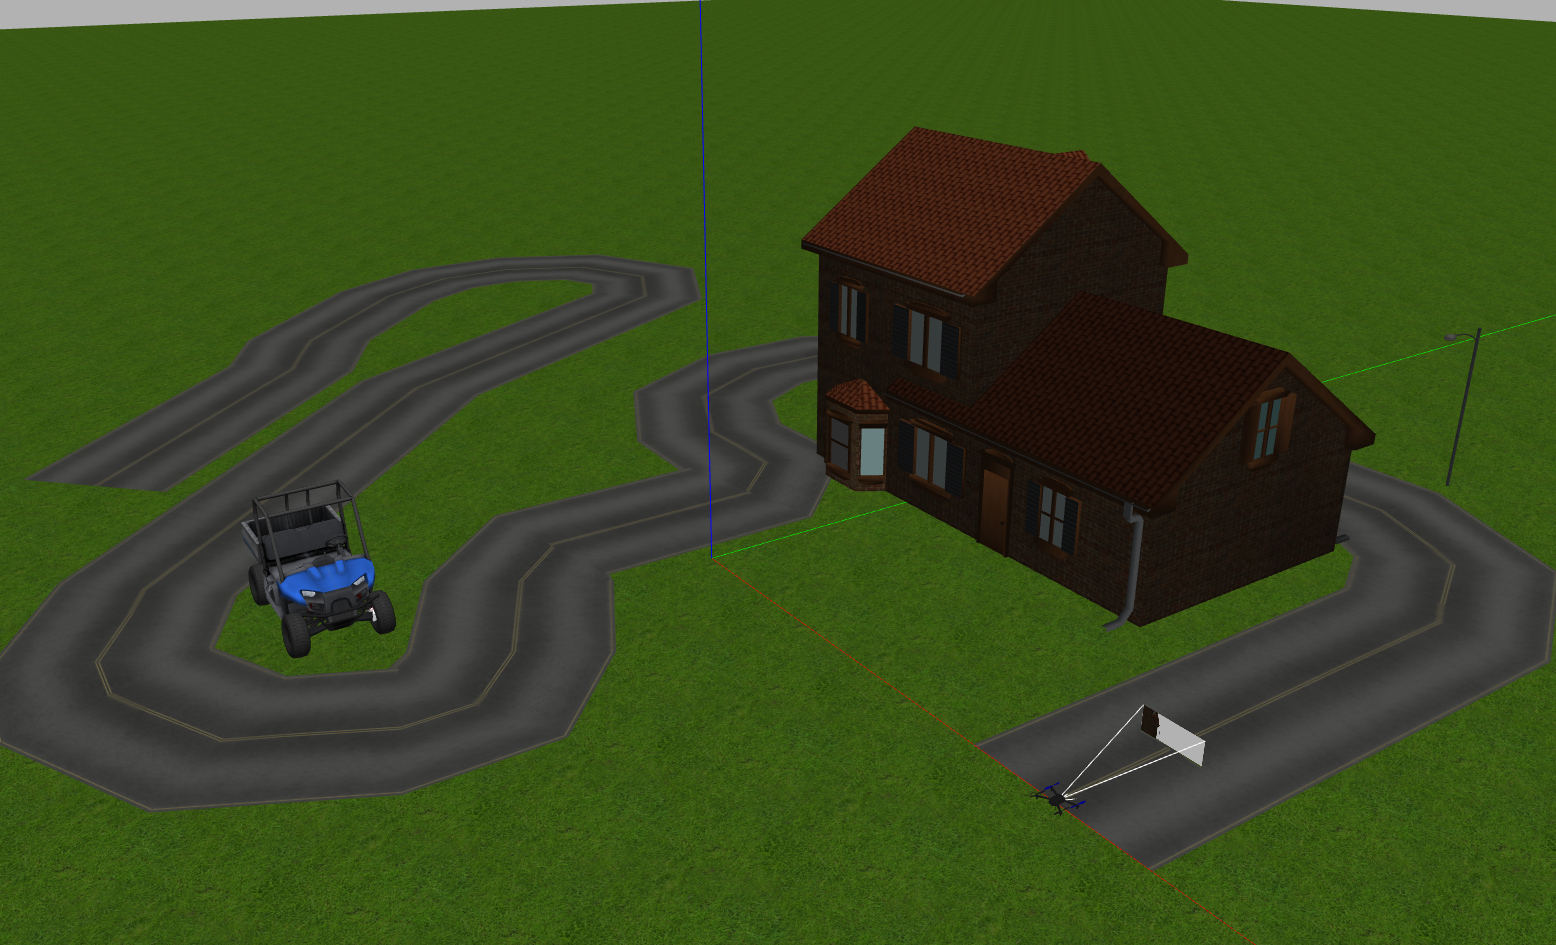
\includegraphics[width=0.7\linewidth]{figures/mundo_fr.png}
		\caption{Escenario de Follow Road}
		\label{fig.mundo_fr}
		\end{center}
\end{figure}

\subsection{Ficheros de configuración} \label{sec.launch_fr}
Para la incorporación del modelo del circuito y del robot, es necesario la creación de un fichero de configuración que importe en \textit{Gazebo} los elementos de los que consta el escenario y su localización. Este fichero tiene la extensión \textit{.world} y \textit{Gazebo} es capaz de leerlo y mostrar el escenario al iniciarse.
El código del fichero es el siguiente:

\lstset{language=XML, breaklines=true, basicstyle=\footnotesize}
\begin{lstlisting}[frame=single]
<?xml version="1.0" ?>
<sdf version="1.5">
  <world name="default">
    <scene>
      <grid>false</grid>
    </scene>

    <include>
      <uri>model://sun</uri>
    </include>
    <include>
      <uri>model://grass_plane</uri>
    </include>

    <include>
      <uri>model://house_4</uri>
      <pose>1 6.43 0 0 0 0</pose>
    </include>
    <include>
      <uri>model://polaris_ranger_ev</uri>
      <pose>-1.48 -6 0.1 0 0 0</pose>
      <static>true</static>
    </include>
    <include>
      <uri>model://lamp_post</uri>
      <pose>5 13 0 0 0 0</pose>
    </include>
    <include>
      <uri>model://lamp_post</uri>
      <pose>-4 13 0 0 0 0</pose>
    </include>
    <include>
      <uri>model://iris_fpv_cam</uri>
      <pose>8 0 0.3 0 0 1.57</pose>
    </include>
    <road name="my_road">
      <width>3</width>

      <point>8 0 0.01</point>
      <point>8 3 0.01</point>
      <point>8 8 0.01</point>
      <point>7 10 0.01</point>
      <point>5 11 0.01</point>
      <point>-5 11 0.01</point>
      <point>-7 10 0.01</point>
      <point>-8 8 0.01</point>
      <point>-8 6 0.01</point>
      <point>-7 4 0.01</point>
      <point>-5 3 0.01</point>
      <point>-3 3 0.01</point>
      <point>-2 2 0.01</point>
      <point>-2 -2 0.01</point>
      <point>-1 -3 0.01</point>

      <point>1 -4 0.01</point>
      <point>2 -5 0.01</point>

      <point>2 -6 0.01</point>
      <point>1 -8 0.01</point>
      <point>-1 -9 0.01</point>
      <point>-2 -9 0.01</point>
      <point>-4 -8 0.01</point>

      <point>-11 -1 0.01</point>
      <point>-14 5 0.01</point>

      <point>-15 7 0.01</point>
      <point>-17 8 0.01</point>
      <point>-19 7 0.01</point>

      <point>-20 5 0.01</point>
      <point>-20 3 0.01</point>
      <point>-19 1 0.01</point>
      <point>-17 -1 0.01</point>

      <point>-16 -2 0.01</point>
      <point>-14 -3 0.01</point>
      <point>-9 -8 0.01</point>
    </road>
  </world>
</sdf>
\end{lstlisting}

Además de este fichero, es necesario un fichero complementario de arranque que importe los \textit{plugins y drivers} de ROS-Kinetic. Este tipo de fichero tienen la extensión \textit{.launch}. En él, se pasan a \textit{Gazebo} argumentos como el nombre del fichero de configuración con el escenario, establecer el tiempo que se va a utilizar en el escenario, la posible ejecución de un GUI y otras opciones de depuración.
El fichero es el siguiente:

\lstset{language=XML, breaklines=true, basicstyle=\footnotesize}
\begin{lstlisting}[frame=single]
<?xml version="1.0" encoding="UTF-8"?>
<launch>
  <include file="$(find gazebo_ros)/launch/empty_world.launch">
    <arg name="world_name" value="road_drone_textures_ROS.world"/>
    <arg name="paused" value="false"/>
    <arg name="use_sim_time" value="true"/>
    <arg name="gui" value="true"/>
    <arg name="headless" value="false"/>
    <arg name="debug" value="false"/>
    <arg name="verbose" default="true"/>
  </include>

  <arg name="fcu_url" default="udp://:14540@127.0.0.1:14540" />
	<arg name="gcs_url" default="" />
	<arg name="tgt_system" default="1" />
	<arg name="tgt_component" default="1" />
	<arg name="log_output" default="screen" />
	<arg name="fcu_protocol" default="v2.0" />
	<arg name="respawn_mavros" default="false" />

	<include file="$(find mavros)/launch/node.launch">
		<arg name="pluginlists_yaml" value="$(find mavros)/launch/px4_pluginlists.yaml" />
		<arg name="config_yaml" value="$(find mavros)/launch/px4_config.yaml" />

		<arg name="fcu_url" value="$(arg fcu_url)" />
		<arg name="gcs_url" value="$(arg gcs_url)" />
		<arg name="tgt_system" value="$(arg tgt_system)" />
		<arg name="tgt_component" value="$(arg tgt_component)" />
		<arg name="log_output" value="$(arg log_output)" />
		<arg name="fcu_protocol" value="$(arg fcu_protocol)" />
		<arg name="respawn_mavros" default="$(arg respawn_mavros)" />
	</include>

  <node pkg="mavros" type="px4.sh"  name="px4" output="screen"/>
</launch>
\end{lstlisting}

\subsection{Diseño}
El diseño de la infraestructura de esta práctica es distinta de las existentes hasta ahora. Esto se debe a la utilización de paquetes \textit{MavROS} en el dron. Para el funcionamiento del dron con \textit{MavROS}, es necesario el soporte de \textit{MAVLink}. \textit{MAVLink} es un protocolo de comunicación para vehículos aéreos y la estación de tierra. Este protocolo proporciona los mensajes para comunicarse con el dron. 

Apoyado en \textit{MAVLink} se encuentra \textit{MavROS}. Se trata de un nodo de \textit{ROS} que realiza una conversión entre los \textit{topics} que se utilizan en \textit{ROS} para comunicarse con los drones y los mensajes de \textit{MAVLink} permitiendo, de esta manera, la comunicación de los vehículos autónomos con aplicaciones \textit{ROS}. Además, proporciona los \textit{topics} finales del dron.

En cuanto al control de bajo nivel del dron, se ha utilizado el software libre \textit{Px4}. Se trata de un sistema de pilotaje automático de drones especialmente orientado a pilotaje fuera de la línea de visión del usuario. Este \textit{software} aporta la infraestructura básica del dron y corre como plugins de Gazebo (Figura \ref{fig.diseno_fr}).

\begin{figure}[H]
  \begin{center}
    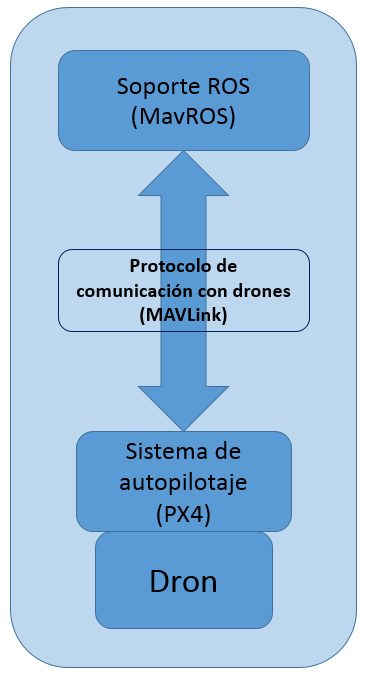
\includegraphics[width=6.5cm, height=7.3cm]{figures/diseno_fr.png}
		\caption{Diseño de la infraestructura del ejercicio}
		\label{fig.diseno_fr}
		\end{center}
\end{figure} 

\section{Plantilla de nodo ROS}
Una vez explicada la infraestructura de la práctica, en esta sección se va a explicar la plantilla de nodo ROS desarrollada. Esta plantilla es una manera de ejecutar los ejercicios de \textit{Robotics-Academy} (Figura \ref{fig.na_fr}). Esta plantilla de nodo ROS de la práctica, está formada por:

\begin{itemize}
    \item Fichero principal.
    \item Fichero de solución
    \item GUI. Directorio con todos los ficheros para el funcionamiento del GUI.
\end{itemize}

El fichero principal es el código que va a ejecutarse al lanzar el nodo académico de la práctica. En él se especifican las conexiones con los \textit{topics} que se van a establecer, así como la inicialización del GUI.

En el fichero de solución hay un conjunto de funciones que aportan la funcionalidad de la práctica, como comenzar, parar, recoger imagen, así como las que desarrolle el alumno y el propio código con la solución de referencia.

\begin{figure}[H]
  \begin{center}
    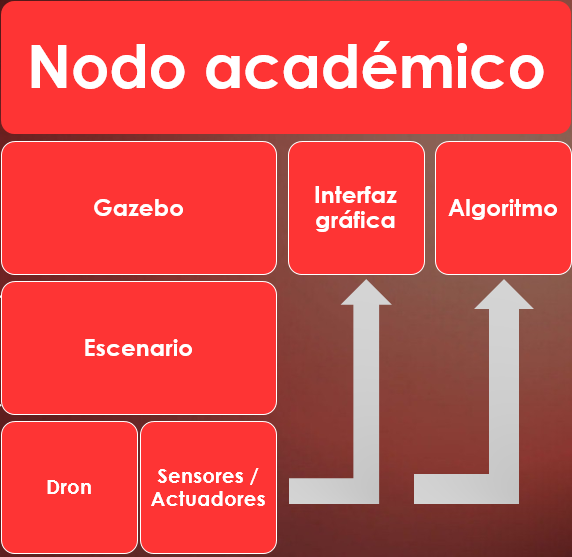
\includegraphics[width=0.9\textwidth, height=8cm]{figures/na_fr.png}
		\caption{Plantilla de nodo ROS del ejercicio Follow\_Road}
		\label{fig.na_fr}
		\end{center}
\end{figure} 

\subsection{Arquitectura software}
Esta práctica tiene tres hilos de ejecución, en lugar de uno monolítico, para aliviar la carga computacional. De esta manera se aumenta la velocidad a la que puede trabajar el simulador \textit{Gazebo} porque se aprovechan mejor los múltiples núcleos que puede tener el ordenador del estudiante.

\begin{itemize}
	\item Hilo de percepción: se encarga de la actualización de los datos de los sensores del robot. Este hilo se comunica con \textit{Gazebo} para recoger datos de la odometría y la cámara y entregárselos al nodo ROS. Además, es el encargado de ejecutar el código del alumno.
	\item Hilo de la interfaz gráfica del usuario (GUI): se encarga del refresco del GUI de la práctica. Esta hebra tiene una carga computacional elevada dado se encarga de refrescar las imágenes obtenidas por las cámaras.
	\item Hilo de control: se encarga de enviar la información del nodo ROS al dron. Se conecta con los \textit{topics}, proporcionados por \textit{MavROS}, para enviar las órdenes de movimiento.
\end{itemize}

\subsection{Interfaz de sensores y actuadores}
Tanto para recoger los datos de los sensores como para enviar los datos de los actuadores, el nodo ROS proporciona un HAL-API de interconexión con los \textit{topics}. De esta manera, es sobre esta interfaz sobre la que el alumno debe apoyarse para desarrollar su algoritmo, dejando los detalles de más bajo nivel transparentes para el mismo. EL HAL-API proporcionado por este nodo ROS es el siguiente:
\begin{itemize}
    \item self.drone.getPose3d(): con esta función se obtiene la odometría del dron.
    \item self.drone.getImage(): con esta función se obtienen las imágenes captadas por la cámara.
    \item self.drone.sendCMDVel(): con esta función se envía las velocidades y el giro del dron.
\end{itemize}

Para realizar las conexiones a los \textit{topics} ofrecidos por \textit{MavROS} con el HAL-API proporcionado al estudiante, se han desarrollado unos recubrimientos que permiten un fácil acceso desde el código del estudiante a los \textit{ROS-topics} que ofrece el nodo \textit{MavROS} para gobernar al dron. Para ello se han creado un total de seis ficheros con código en \textit{Python} que dotan de la infraestructura necesaria, al nodo ROS, para comunicarse con el dron.

\begin{itemize}
    \item En el fichero \textit{\_\_init\_\_.py}, se establecen las cabeceras de las funciones principales de interconexión y las conexiones de los \textit{topics}.
    \item En el fichero \textit{camera.py}, se han desarrollado las funciones necesarias para recoger las imágenes captadas por las cámaras integradas en el dron.
    \item En el fichero \textit{cmdvel.py}, se incorporan las funciones necesarias para enviar los comandos de velocidad al plugin de \textit{MavROS}.
    \item En el fichero \textit{extra.py}, se han desarrollado las funciones para controlar el despegue y aterrizaje del dron.
    \item En el fichero \textit{pose3d.py}, están las funciones para recoger la información sobre la odometría del dron.
    \item En el fichero \textit{threadPublisher.py}, está la función de creación de la hebra para las comunicaciones de las hebras de publicación de \textit{topics}.
\end{itemize}

\subsection{Interfaz gráfica}
La interfaz gráfica del usuario (GUI) se utiliza para representar información relacionada con los sensores del robot. Además, permite teleoperar el robot y lanzar/detener la ejecución del algoritmo programado por el estudiante. Esto es muy útil para la depuración, ya que permite la visualización de las órdenes que genera el algoritmo al robot y comprobar su movimiento.

Esta GUI (Figura \ref{fig.guifr}) está formada por tres conjuntos de \textit{widgets}, uno para el visionado de las imágenes, otro para el control del dron y otro para el teleoperador.

\begin{figure}[H]
  \begin{center}
    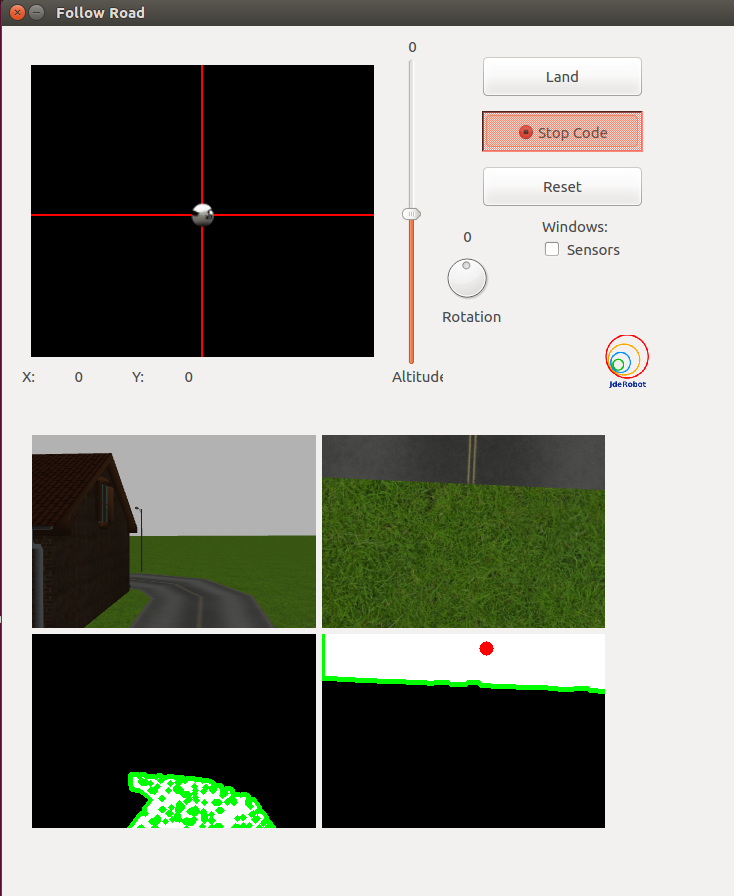
\includegraphics[width=7cm,height=10cm,\textwidth]{figures/GUI_fr.png}
		\caption{Interfaz Gráfica Folow\_Road}
		\label{fig.guifr}
		\end{center}
\end{figure}

El \textit{widget} del teleoperador se utiliza para controlar el dron una vez ha despegado. De esta manera se puede comprobar que las conexiones del dron están correctamente realizadas.

El conjunto \textit{widgets} destinados al control del dron se dividen en tres subconjuntos. Con ellos se puede controlar el dron de manera manual:
\begin{itemize}
    \item Control de altitud y rotación.
    \item widgets de estabilización.
    \item Botón de despegue/aterrizaje, botón de ejecución y parada del algoritmo de solución y botón de reinicio del puntero del teleoperador.
\end{itemize}

El \textit{widget} de visionado del dron incorpora cuatro pantallas. Las pantallas superiores reflejan las imágenes recogidas por las cámaras del dron y las pantallas inferiores muestran el procesado de las imágenes realizado en el algoritmo de solución del alumno. Este \textit{widget} es muy útil para depurar el código del alumno ya que puede verse, fácilmente, el resultado de su procesado a la imagen.

El último conjunto de \textit{widgets} lo forman los botones de control del algoritmo. Con ellos puedes ejecutar y detener el algoritmo desarrollado, despegar y aterrizar el dron y reiniciar la posición del teleoperador.

\section{Solución de referencia}
Para esta práctica se ha desarrollado una solución de referencia compatible con \textit{ROS} y \textit{OpenCV} que consta de una parte perceptiva de procesamiento de imagen y una parte de control de movimiento.

\subsection{Procesamiento de imagen}
El procesamiento de las imágenes programado se ha realizado en función del contorno del filtrado. Este procedimiento es similar al realizado en la solución de referencia de la práctica anterior con la diferencia del filtrado de la carretera en lugar de una línea roja. 

Se comienza con la recogida de las imágenes captadas por la cámara y obteniendo la imagen HSV\footnote{\url{https://es.wikipedia.org/wiki/Modelo_de_color_HSV}} para poder filtrar la carretera. Tras obtener la imagen HSV, podemos seleccionar el rango de valores que componen color de la carretera como un array con la intensidad mínima y máxima del color y se filtra la imagen con los rangos de color para obtener la carretera.

\lstset{language=Python, breaklines=true, basicstyle=\footnotesize}
\begin{lstlisting}[frame=single]
input_imageV = self.drone.getImageVentral().data
input_imageF = self.drone.getImageFrontal().data

image_HSV_V = cv2.cvtColor(input_imageV, cv2.COLOR_RGB2HSV)
image_HSV_F = cv2.cvtColor(input_imageF, cv2.COLOR_RGB2HSV)

value_min_HSV = np.array([20, 0, 0])
value_max_HSV = np.array([100, 130, 130])

image_HSV_filtered_V = cv2.inRange(image_HSV_V, value_min_HSV, value_max_HSV)
image_HSV_filtered_F = cv2.inRange(image_HSV_F, value_min_HSV, value_max_HSV)
\end{lstlisting}

La modificación del resto del algoritmo, con respecto a la práctica anterior es la introducción de técnicas de eliminación de ruido (opening y closing) en las imágenes filtradas. 

\lstset{language=Python, breaklines=true, basicstyle=\footnotesize}
\begin{lstlisting}[frame=single]
opening_V = cv2.morphologyEx(image_HSV_filtered_V, cv2.MORPH_OPEN, np.ones((5,5),np.uint8))
closing_V = cv2.morphologyEx(opening_V, cv2.MORPH_CLOSE, np.ones((10,10),np.uint8))

opening_F = cv2.morphologyEx(image_HSV_filtered_F, cv2.MORPH_OPEN, np.ones((5,5),np.uint8))

image_HSV_filtered_Mask_V = np.dstack((closing_V, closing_V, closing_V))
image_HSV_filtered_Mask_F = np.dstack((opening_F, opening_F, opening_F))

imgray_V = cv2.cvtColor(image_HSV_filtered_Mask_V, cv2.COLOR_BGR2GRAY)
ret_V, thresh_V = cv2.threshold(imgray_V, 127, 255, 0)
_, contours_V, hierarchy_V = cv2.findContours(thresh_V, cv2.RETR_TREE, cv2.CHAIN_APPROX_SIMPLE)
cv2.drawContours(image_HSV_filtered_Mask_V, contours_V, -1, (0,255,0), 3)

imgray_F = cv2.cvtColor(image_HSV_filtered_Mask_F, cv2.COLOR_BGR2GRAY)
ret_F, thresh_F = cv2.threshold(imgray_F, 127, 255, 0)
_, contours_F, hierarchy_F = cv2.findContours(thresh_F, cv2.RETR_TREE, cv2.CHAIN_APPROX_SIMPLE)
cv2.drawContours(image_HSV_filtered_Mask_F, contours_F, -1, (0,255,0), 3)
\end{lstlisting}

Tras dibujar el contorno de la sección, es necesaria una comprobación del filtrado de la imagen para evitar errores en la ejecución. En el caso de haber más de una zona que pase el filtro debe escoger la adecuada. Una vez hechas estas comprobaciones, se extrae el centro de la zona filtrada y se dibuja un punto rojo

\lstset{language=Python, breaklines=true, basicstyle=\footnotesize}
\begin{lstlisting}[frame=single]
area = []
for pic, contour in enumerate(contours_V):
    area.append(cv2.contourArea(contour))

if len(area) > 1:
    if area[0] < area[1]:
        M = cv2.moments(contours_V[1])
    else:
        M = cv2.moments(contours_V[0])

else:
    try:
        M = cv2.moments(contours_V[0])
    except IndexError:
        self.drone.sendCMDVel(0,0.3,0,0)
        M = cv2.moments(0)

if int(M['m00']) != 0:
    cx = int(M['m10']/M['m00'])
    cy = int(M['m01']/M['m00'])

cv2.circle(image_HSV_filtered_Mask_V, (cx, cy), 7, np.array([255, 0, 0]), -1)
\end{lstlisting}

Para visualizar en el GUI el procesado de las imágenes se utilizan las siguientes instrucciones:

\lstset{language=Python, breaklines=true, basicstyle=\footnotesize}
\begin{lstlisting}[frame=single]
self.setImageFilteredVentral(image_HSV_filtered_Mask_V)
self.setImageFilteredFrontal(image_HSV_filtered_Mask_F)
\end{lstlisting}

\subsection{Control de movimiento}
Una vez procesada la imagen, es posible controlar el dron con el punto del centro de la sección obtenido. De esta manera, el dron se limitará a seguir dicho punto, adecuando sus movimientos hacia el mismo.

\lstset{language=Python, breaklines=true, basicstyle=\footnotesize}
\begin{lstlisting}[frame=single]
if cy > 120:
    self.drone.sendCMDVel(0,0.3,0,0.2)
    print("Turning")
elif cx < 20:
    print("Detected two roads")
    self.drone.sendCMDVel(0,0.3,0.1,0.0)
else:
    self.drone.sendCMDVel(0,0.3,0,0.0)

print("cx: " + str(cx) + " cy: " + str(cy))
self.yaw = int(cx)
\end{lstlisting}

\section{Validación experimental}
La optimización de los algoritmos anteriores ha sido posible gracias a la realización de diversos experimentos. Estos experimentos han hecho salir a la luz errores en el algoritmo desarrollado que han sido subsanados.
Además, se han realizado experimentos globales donde se ha validado la práctica en su totalidad, nodo académico, infraestructura de la práctica y solución desarrollada.

Se ha preparado un documento \textit{README.md}, incluido en la infraestructura de la práctica, que sirve de guía al alumno a la hora de ejecutar la práctica. En él se incluye información acerca de su ejecución, la API de los sensores y actuadores de ROS e, incluso, un vídeo demostrativo con una ejecución\footnote{\url{https://www.youtube.com/watch?v=76QNSUGXFT8}}.

Para ejecutar al práctica es necesario lanzar en una terminal el fichero de configuración de ROS, llamado \textit{follow\_road.launch}, descrito en la sección \ref{sec.launch_fr}. Para lanzar el fichero hay que ejecutar el siguiente comando:

\lstset{language=bash, breaklines=true, basicstyle=\footnotesize}
\begin{lstlisting}[frame=single]
roslaunch follow_road.launch
\end{lstlisting}

Una vez lanzado el comando en la terminal, se abrirá el simulador \textit{Gazebo} con el escenario del circuito (Figura \ref{fig.circuito}).

\begin{figure}[H]
  \begin{center}
    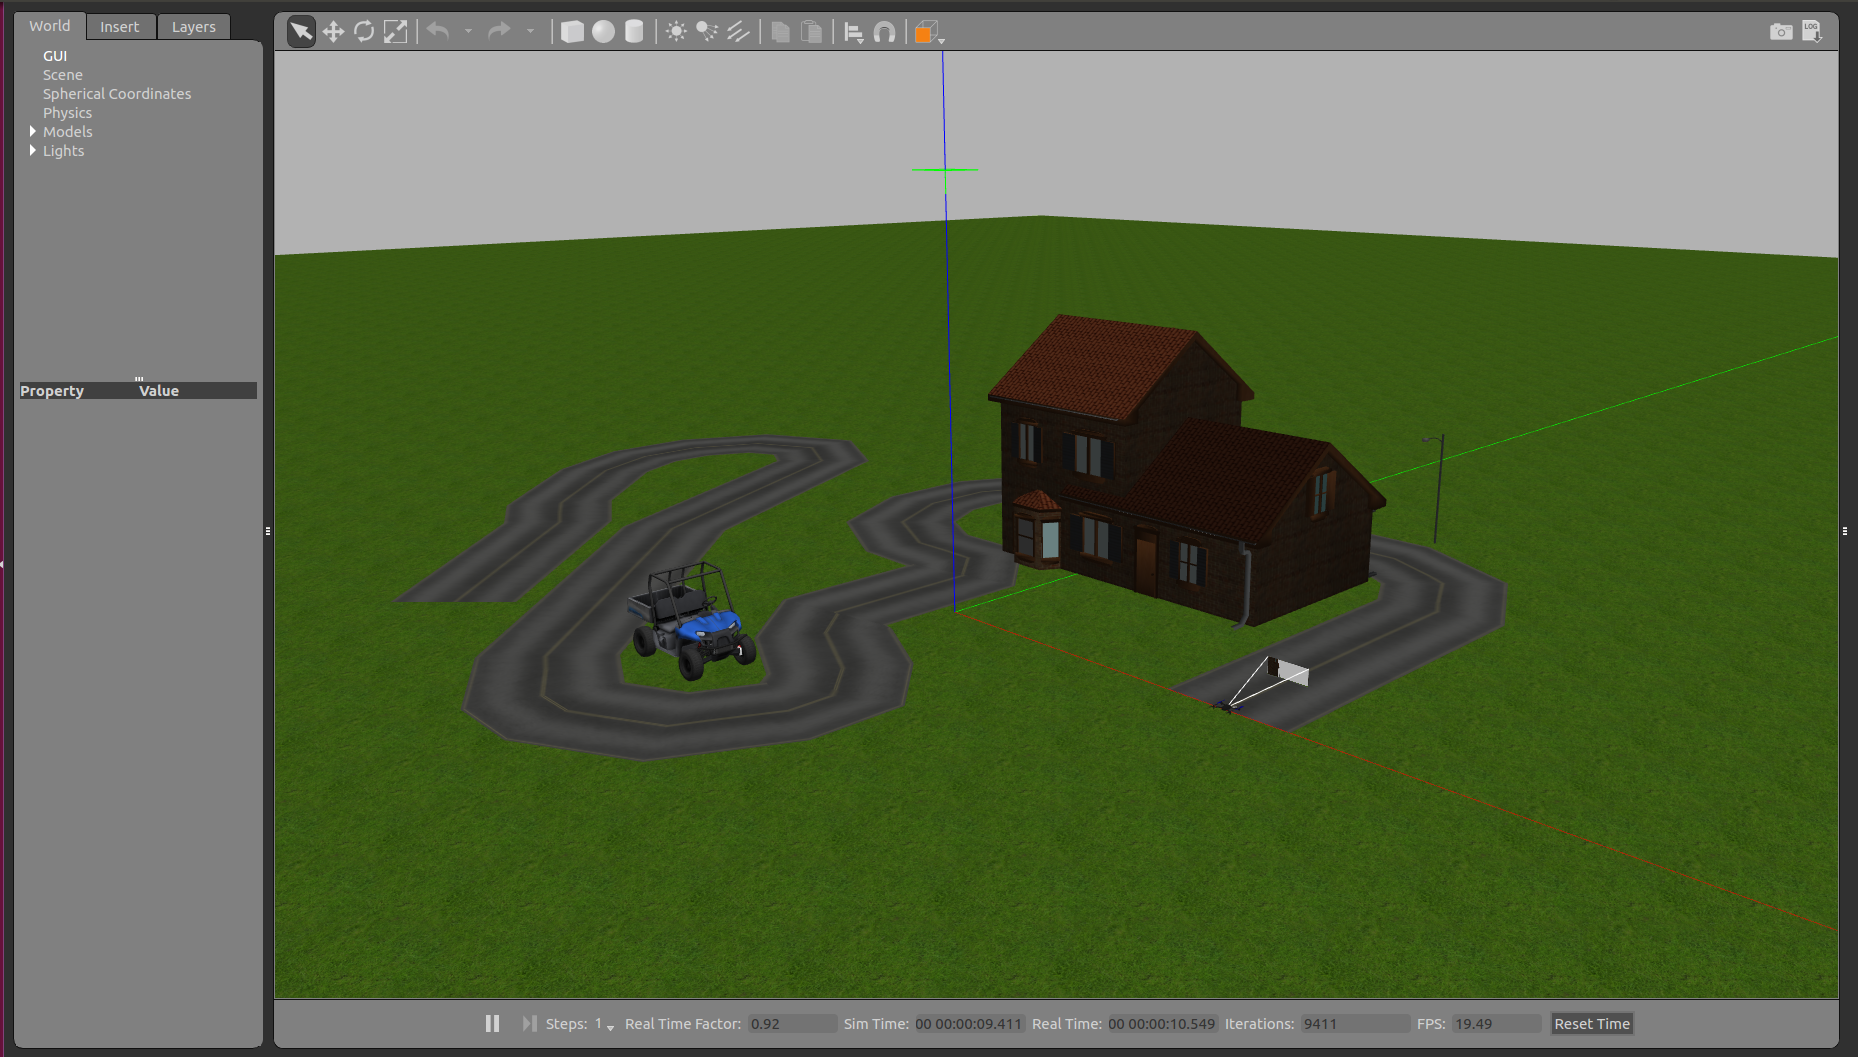
\includegraphics[width=0.98\textwidth]{figures/roslaunch_fr.png}
		\caption{Inicialización de ROS y Gazebo}
		\label{fig.roslaunchfr}
		\end{center}
\end{figure}

Para iniciar el nodo ROS, será necesario ejecutar otro comando en una terminal distinta:

\lstset{language=bash, breaklines=true, basicstyle=\footnotesize}
\begin{lstlisting}[frame=single]
cd ~/Academy/exercises/follow\_road
python2 follow\_road.py
\end{lstlisting}

Una vez ejecutado el comando, el componente académico enlazará los sensores y actuadores proporcionados por \textit{ROS-Kinetic} mediante el fichero de configuración lanzado previamente a la variable \textit{self.drone} que contiene las variables:

\begin{itemize}
    \item self.cameraVentral
    \item self.cameraFrontal
    \item self.pose3d
    \item self.cmdvel
    \item self.extra
\end{itemize}

Con la variable \textit{self.drone}, el nodo ROS se comunica con los \textit{drivers} de \textit{ROS-Kinetic}.
Además de realizar la conexión con los sensores y actuadores, al ejecutar la instrucción, nos aparecerá la interfaz gráfica de usuario (GUI) en la que se podrá visualizar las imágenes recogidas por la cámara, los botones de control y el teleoperador (Figura \ref{fig.inaGfr}).

\begin{figure}[H]
  \begin{center}
    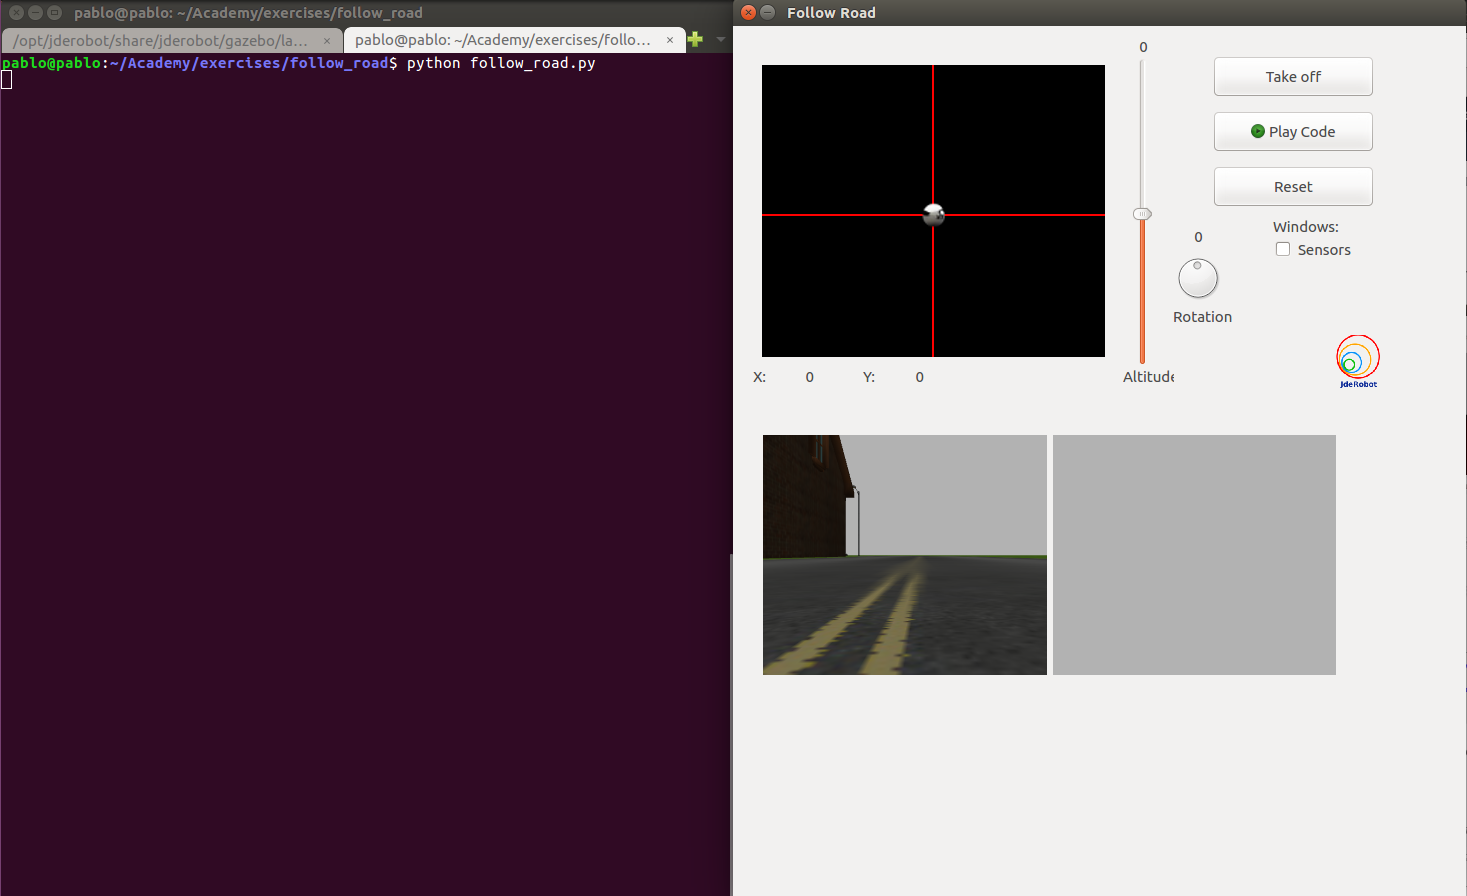
\includegraphics[width=0.98\textwidth]{figures/init_na_fr.png}
		\caption{Inicialización del escenario y el GUI}
		\label{fig.inaGfr}
		\end{center}
\end{figure}

Una vez inicializados los \textit{drivers de ROS-Kinetic}, el escenario en el simulador y el nodo académico, con su GUI, se puede iniciar el algoritmo desarrollado por el alumno. Para ello, es necesario despegar el dron con el botón ``TakeOff'' (Figura \ref{fig.eefr}).

\begin{figure}[H]
  \begin{center}
    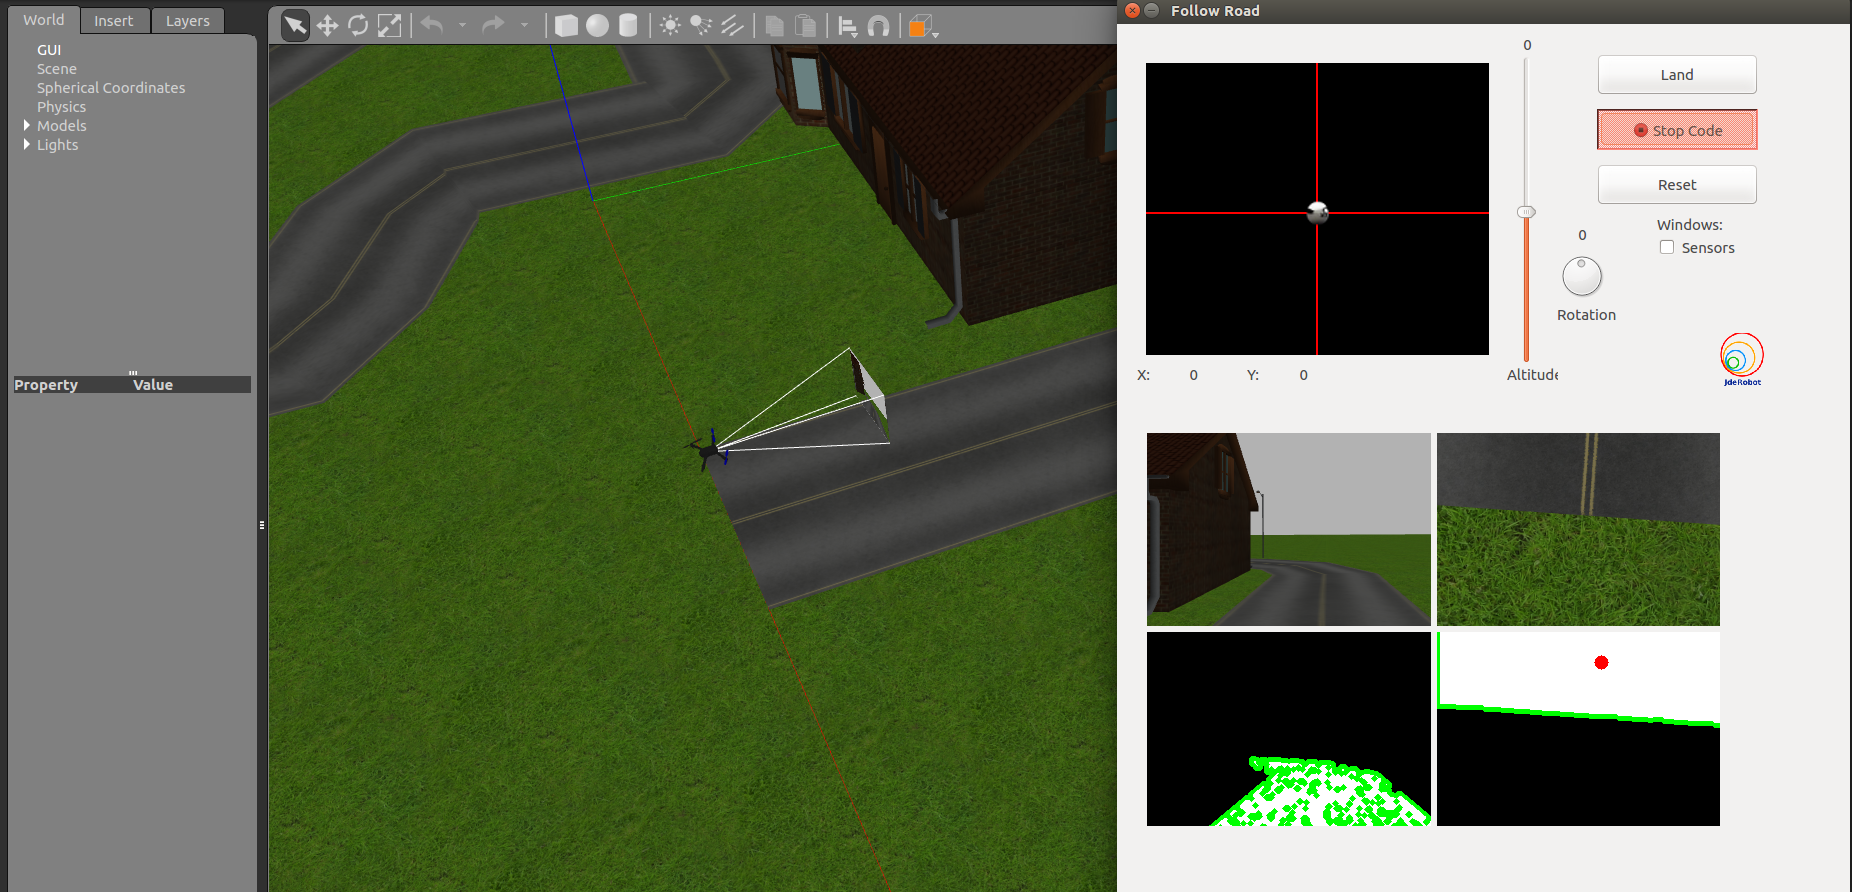
\includegraphics[width=0.98\textwidth]{figures/ejec_estat_fr.png}
		\caption{Ejecución de la práctica}
		\label{fig.eefr}
		\end{center}
\end{figure}

Tras el despegue del dron, se puede lanzar el algoritmo programado con el botón ``Play Code'' (Figuras \ref{fig.etelfr} y \ref{fig.ealgfr}).

\begin{figure}[H]
  \begin{center}
    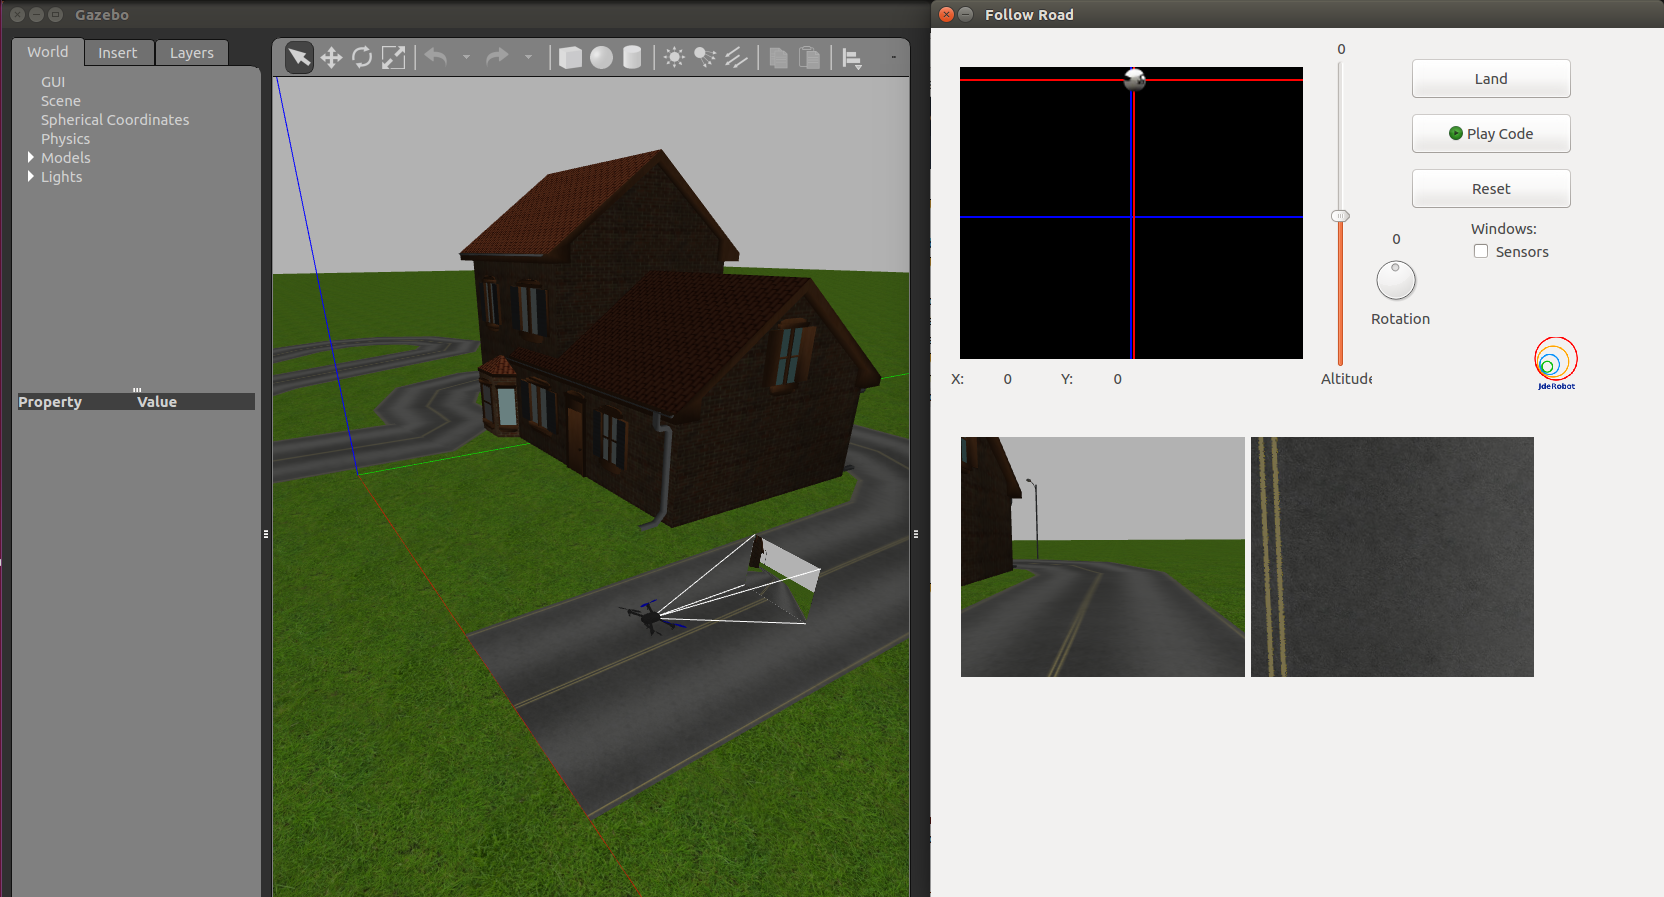
\includegraphics[width=0.98\textwidth]{figures/ejec_teleop_fr.png}
		\caption{Ejecución con teleoperador}
		\label{fig.etelfr}
		\end{center}
\end{figure}

\begin{figure}[H]
  \begin{center}
    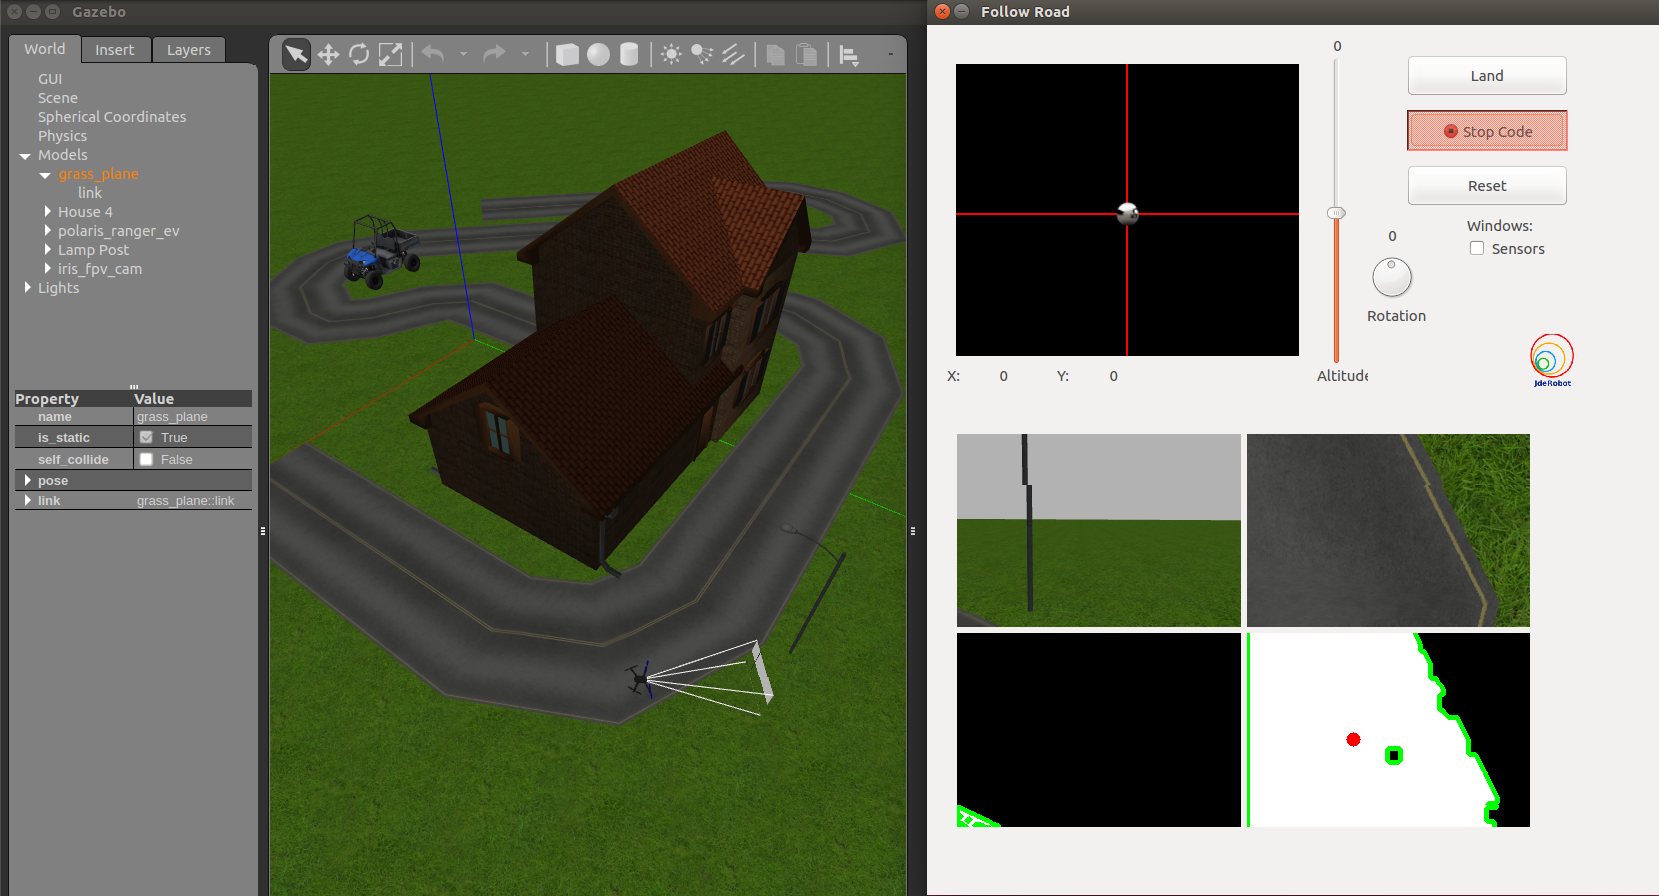
\includegraphics[width=0.98\textwidth]{figures/ejec_algoritmo_fr.png}
		\caption{Ejecución con la solución de la práctica}
		\label{fig.ealgfr}
		\end{center}
\end{figure}

\section{Plantilla del cuadernillo Jupyter}
Como parte paralela a la práctica incluida en \textit{Robotics-Academy}, se ha desarrollado otra plantilla diferente para el mismo ejercicio con cuadernillos de \textit{Jupyter}, en lugar de nodo ROS. Gracias a esto el alumno puede programar y ejecutar el código mediante la utilización del navegador web que prefiera.

Esto supone un paso importante hacia la multiplataforma del entorno docente
\textit{Robotics-Academy}, dado que el alumno puede acceder a las prácticas desde el sistema operativo que prefiera, sólo necesita acceso a internet.

Ha sido necesaria una reestructuración del nodo ROS y de los ficheros que lo componen, además del método para el desarrollo del algoritmo. Se ha eliminado el GUI del nodo ROS y se han introducido los hilos de percepción y control en el cuadernillo de Jupyter. De esta manera, el alumno sólo debe rellenar una celda del cuadernillo con el algoritmo desarrollado.

\begin{figure}[H]
  \begin{center}
    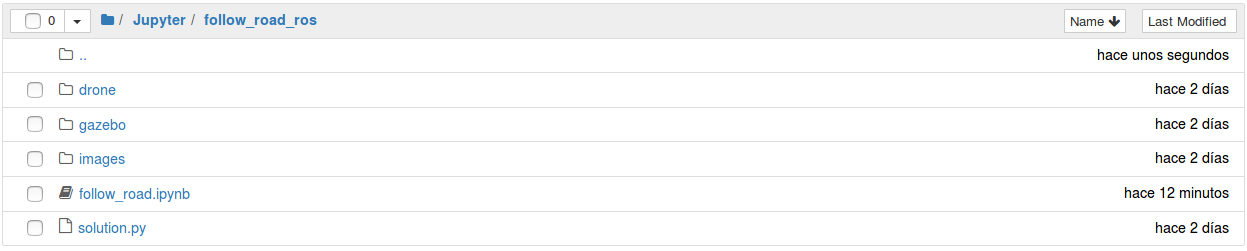
\includegraphics[width=0.98\textwidth]{figures/estructura_jupyter_fr.png}
		\caption{Estructura de la plantilla de Jupyter de la práctica Follow\_Road}
		\label{fig.ejfr}
		\end{center}
\end{figure}

El cuadernillo tiene la estructura de la Figura \ref{fig.ejfr}. Como puede verse, es diferente a la estructura presente en el nodo ROS de Robotics-Academy. Ahora se divide en los siguientes ficheros y carpetas:
\begin{itemize}
    \item images: en este directorio aparecen las imágenes contenidas en el cuadernillo.
    \item gazebo: en este directorio está el fichero de configuración con el escenario y los \textit{drivers}.
    \item interfaces: en este directorio se encuentran los \textit{drivers} de \textit{ROS-Kinetic}.
    \item chrono.ipynb: este fichero es el cuadernillo ejecutable en Jupyter.
\end{itemize}

Para acceder a la práctica, el alumno debe iniciar Jupyter introduciendo en la terminal el siguiente comando:

\lstset{language=bash, breaklines=true, basicstyle=\footnotesize}
\begin{lstlisting}[frame=single]
cd ~/Jupyter
jupyter-notebook
\end{lstlisting}

Con esto se abrirá el navegador web por defecto en la carpeta local Jupyter. Una vez hecho esto, navegaremos hacia el directorio de la práctica de Jupyter ``Follow\_Road'' y abriremos el fichero ``follow\_road.ipynb''. Tras esto se mostrará la siguiente imagen del cuadernillo:

\begin{figure}[H]
  \begin{center}
    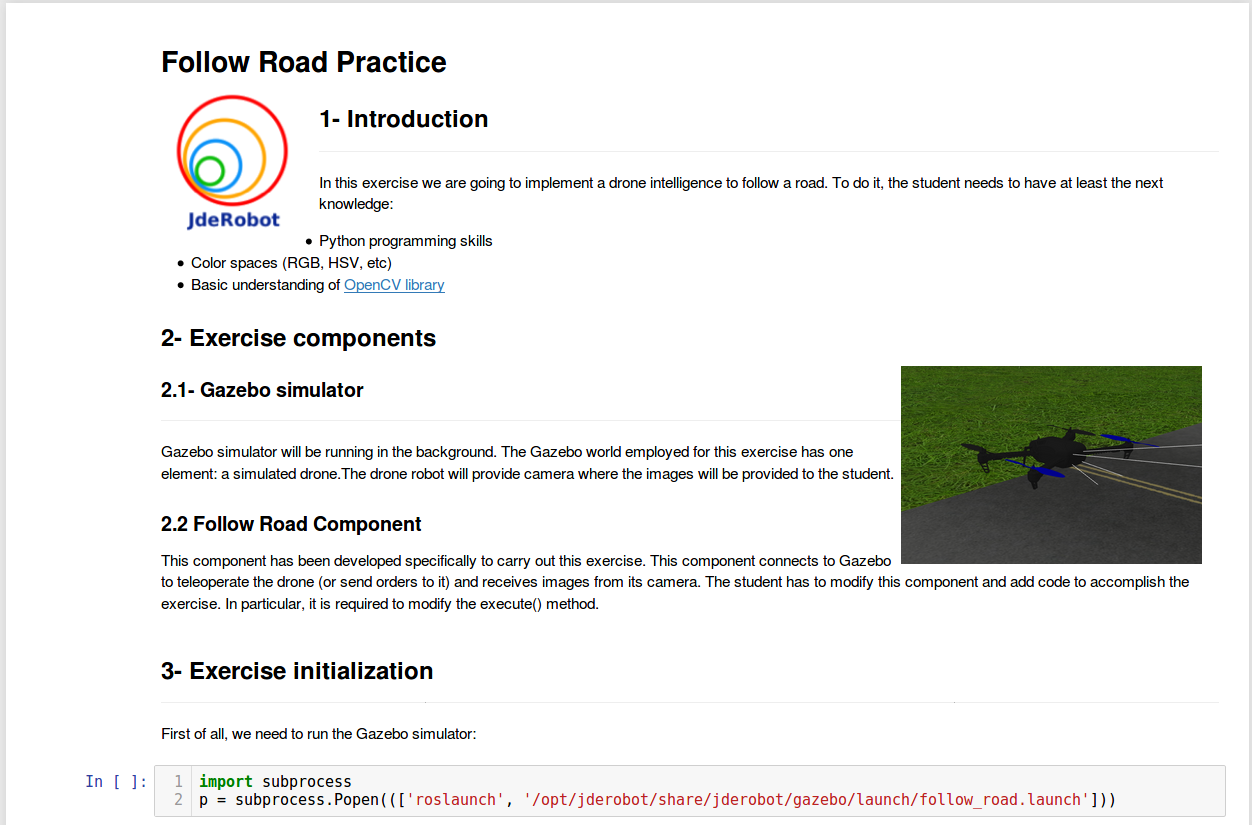
\includegraphics[width=0.98\textwidth]{figures/ipynb_followroad.png}
		\caption{Fichero follow\_road.ipynb}
		\label{fig.ffripynb}
		\end{center}
\end{figure}

El alumno deberá ejecutar las celdas con código y seguir el guión mostrado. En primer lugar, deberá ejecutar el fichero de configuración del mundo que abrirá el escenario (Figura \ref{fig.cmdcfr}).

\begin{figure}[H]
  \begin{center}
    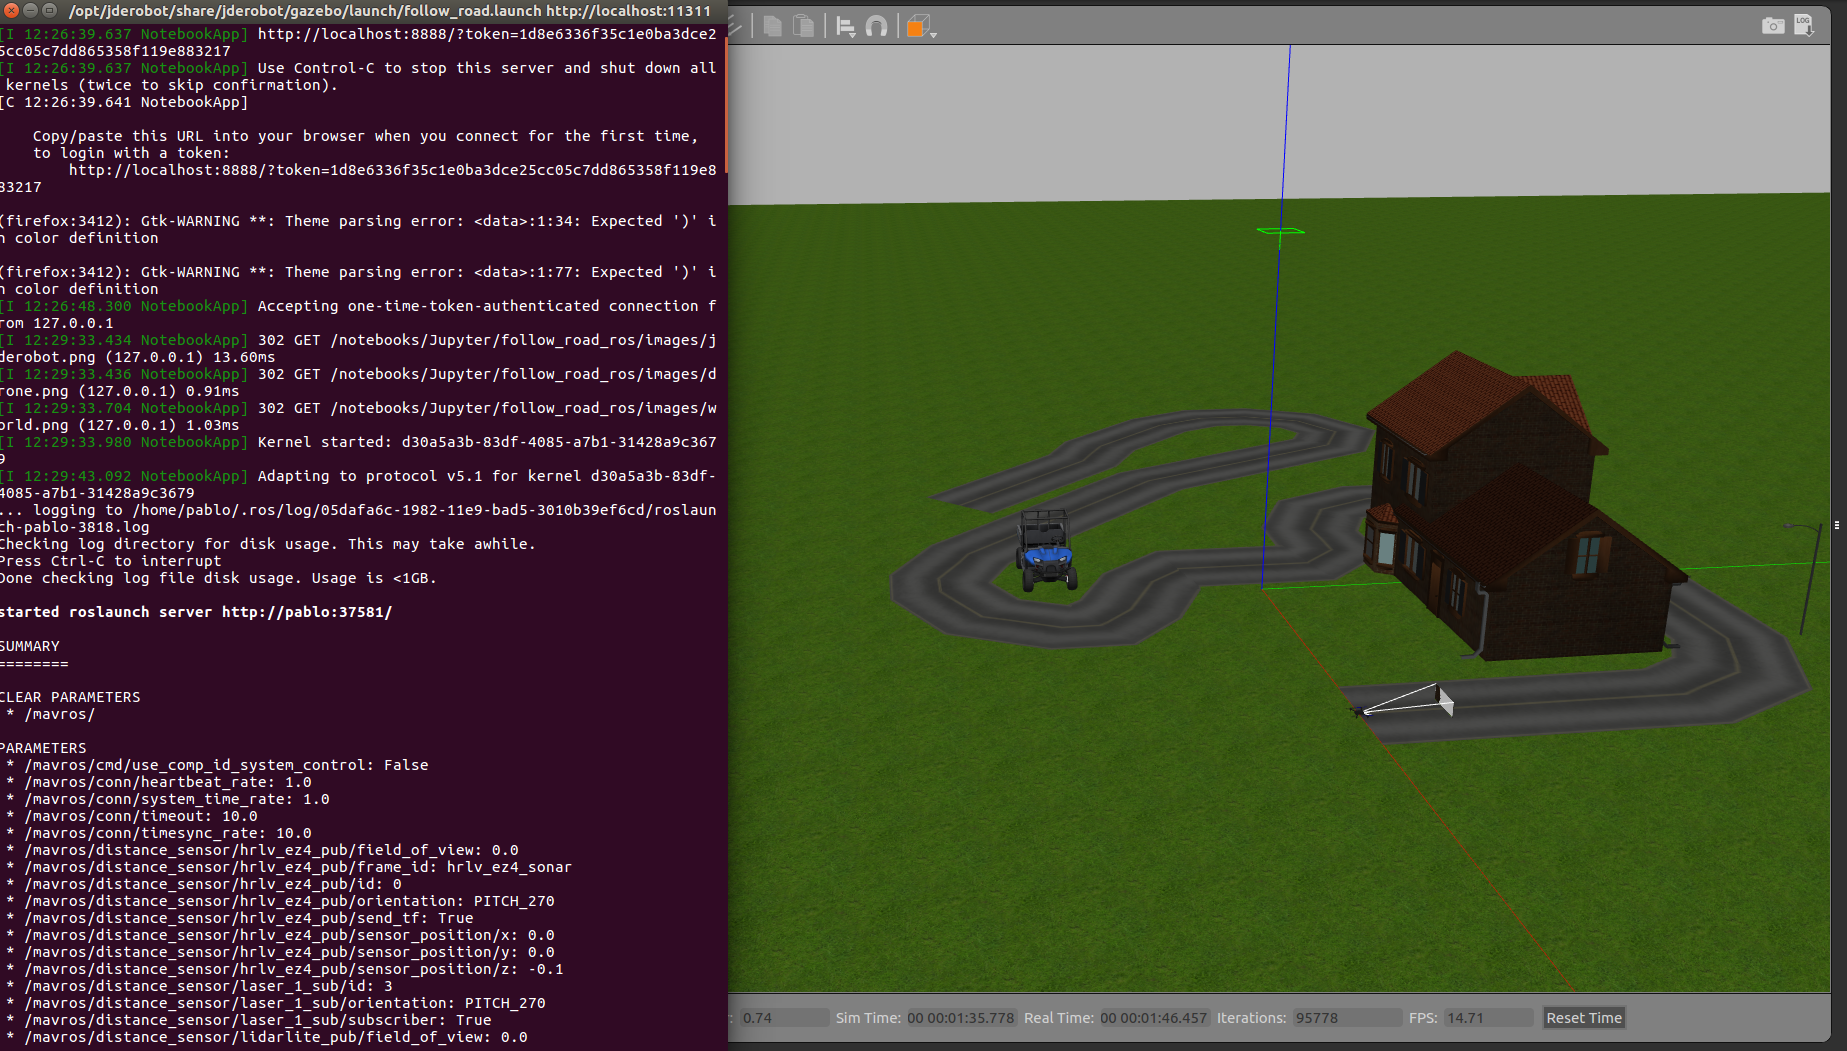
\includegraphics[width=.98\textwidth]{figures/celda_mundo_fr.png}
		\caption{Visualización del mundo}
		\label{fig.cmdcfr}
		\end{center}
\end{figure}

Cuando se haya abierto el simulador es necesario importar el módulo del paquete ``MyAlgorithm.py'' y ``follow\_road.py'' para tener la funcionalidad provista en el nodo ROS. Para ello, se ejecutará la celda correspondiente con las clases ``MyAlgorithm'' y ``FollowRoad''. Una vez importadas, aparece un mensaje de confirmación (Figura \ref{fig.impmafr}).

\begin{figure}[H]
  \begin{center}
    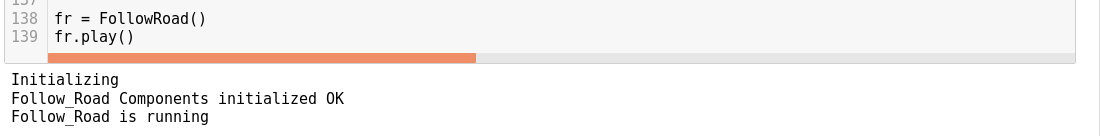
\includegraphics[width=1.2\textwidth]{figures/imp_Ma_FR.png}
		\caption{Importación de las clases ``MyAlgorithm'' y ``FollowRoad''}
		\label{fig.impmafr}
		\end{center}
\end{figure}

Cuando la ejecución imprima el mensaje ``OK'', es necesario despegar el dron (Figura \ref{fig.despfr}).

\begin{figure}[H]
  \begin{center}
    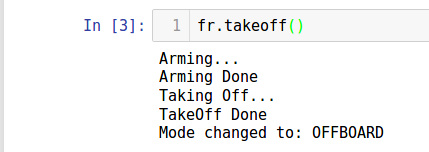
\includegraphics[width=.5\textwidth]{figures/despuegue_fr.png}
		\caption{Despegue del dron}
		\label{fig.despfr}
		\end{center}
\end{figure}

Tras esto, el alumno puede comenzar a programar su código en la celda especificada para ello (Figura \ref{fig.impalg}).

\begin{figure}[H]
  \begin{center}
    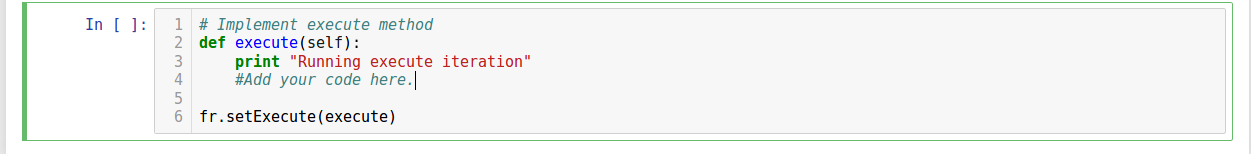
\includegraphics[width=1.5\textwidth]{figures/imp_alg.png}
		\caption{Celda de importación del algoritmo}
		\label{fig.impalg}
		\end{center}
\end{figure}

Una vez ejecutada la celda con el código, aparecerá mensaje iterativo ``Running execute iteration'' (Figura \ref{fig.ecjfr}).

\begin{figure}[H]
  \begin{center}
    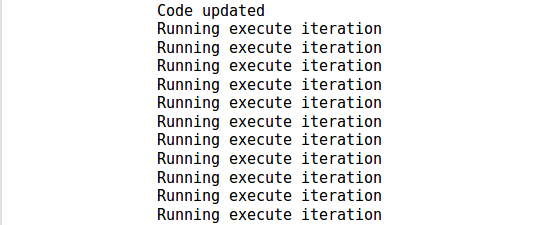
\includegraphics[width=.7\textwidth]{figures/ejec_cod_jup_fr.png}
		\caption{Ejecución del código}
		\label{fig.ecjfr}
		\end{center}
\end{figure}

A continuación, se muestran algunas fotos de la ejecución:

\begin{figure}[H]
  \begin{center}
    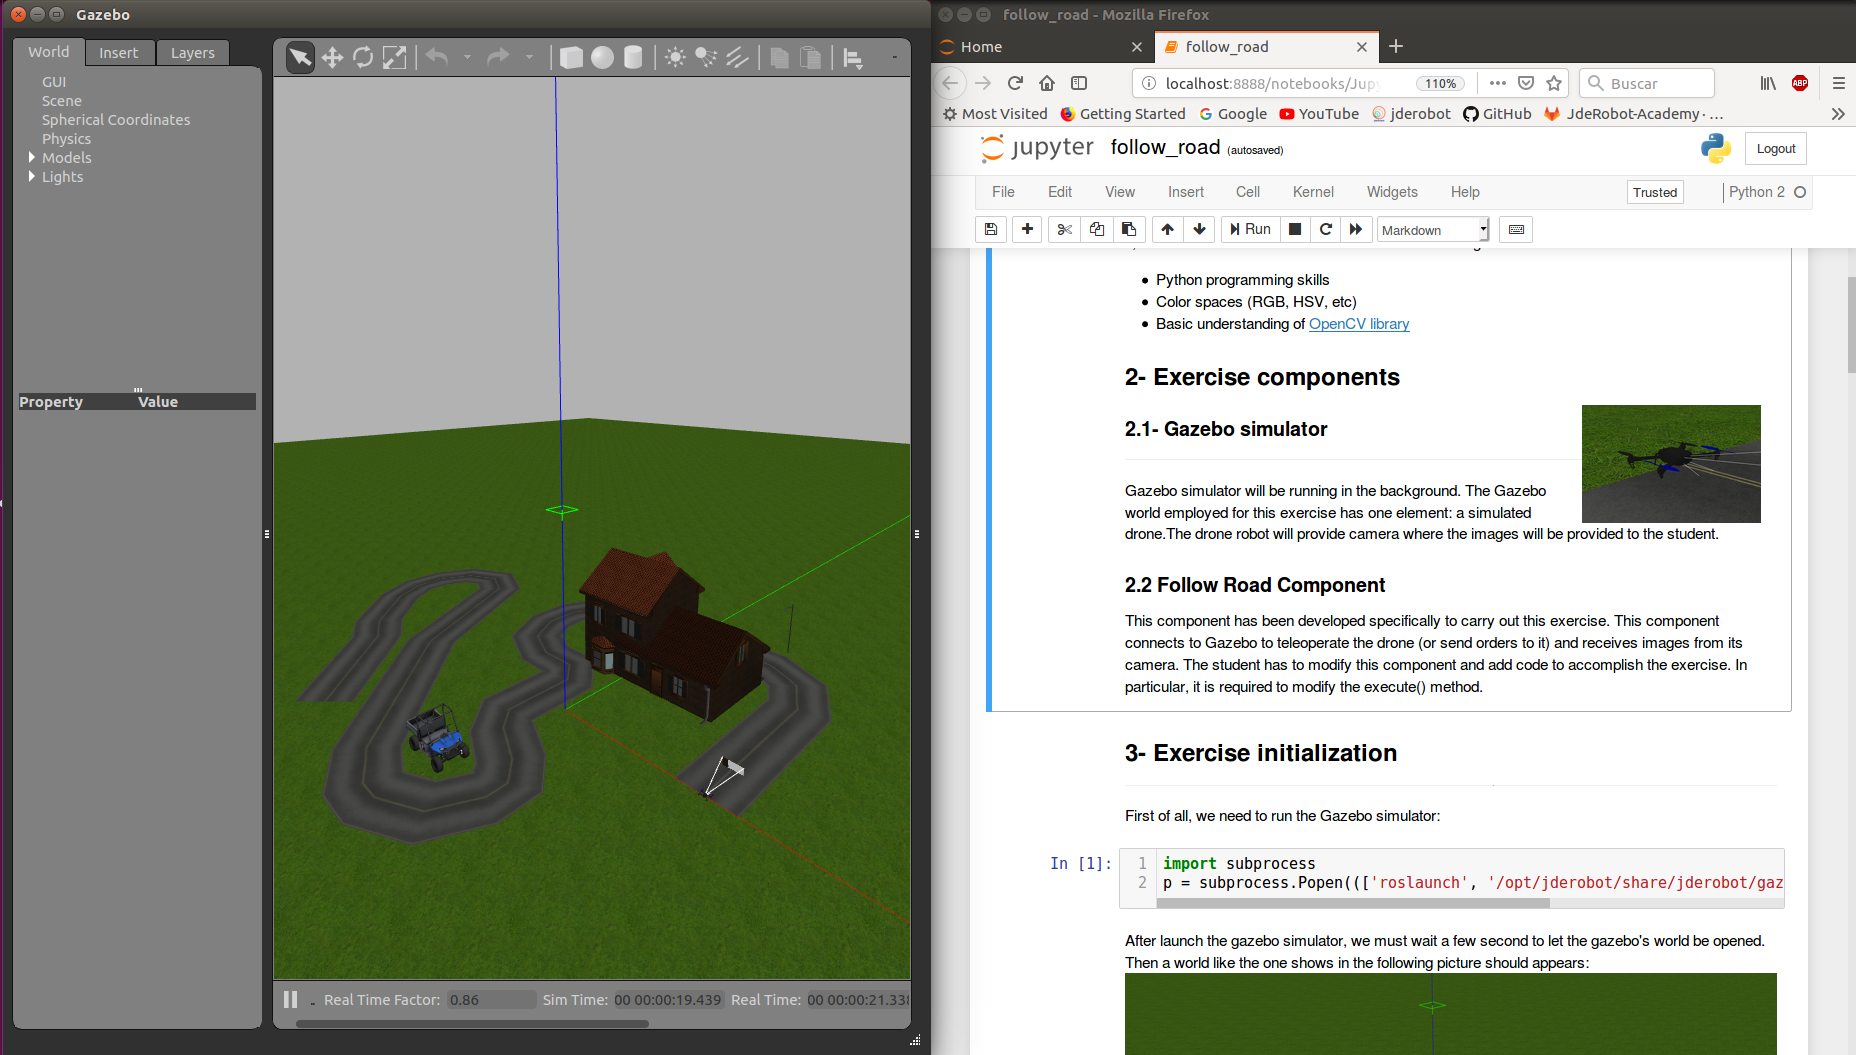
\includegraphics[width=0.7\textwidth]{figures/ejec_1_jup_fr.png}
		\caption{Ejecución del código del ejercicio Follow Road desde un navegador web (a)}
		\label{fig.ecjfr1}
		\end{center}
\end{figure}

\begin{figure}[H]
  \begin{center}
    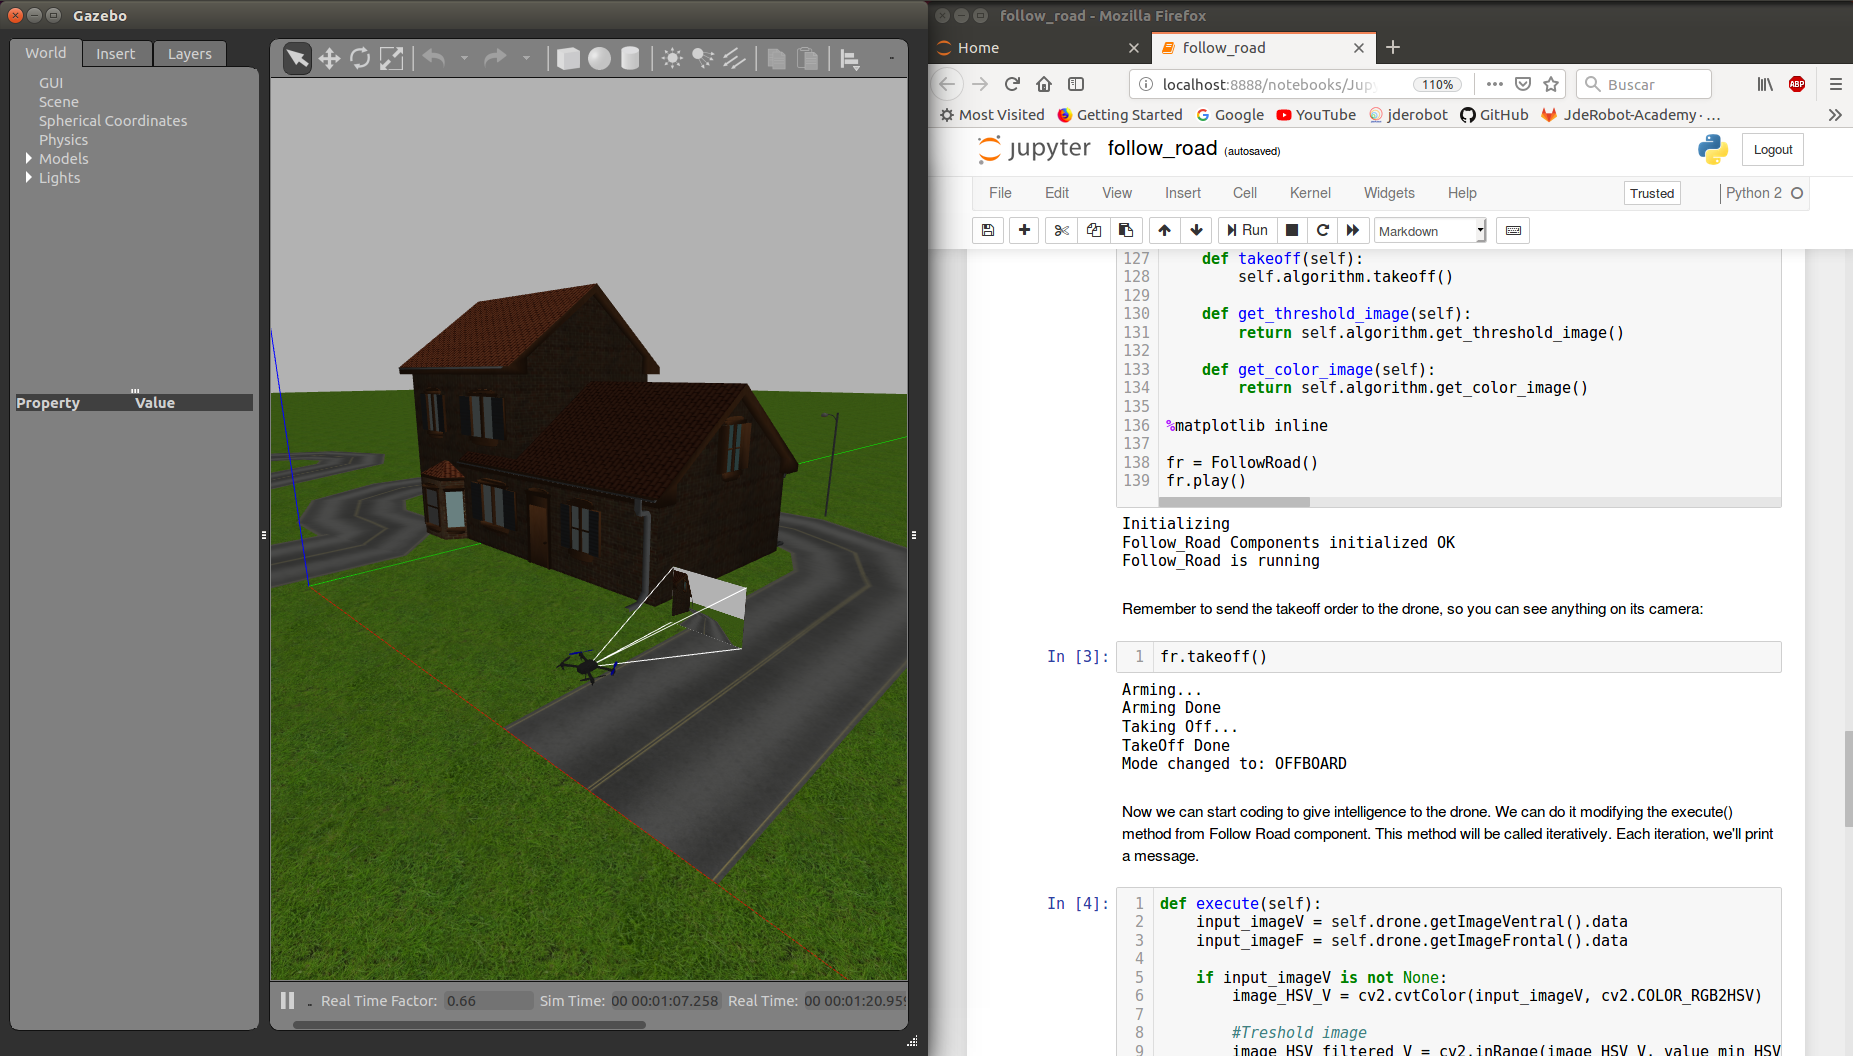
\includegraphics[width=0.7\textwidth]{figures/ejec_2_jup_fr.png}
		\caption{Ejecución del código del ejercicio Follow Road desde un navegador web (b)}
		\label{fig.ecjfr2}
		\end{center}
\end{figure}

\begin{figure}[H]
  \begin{center}
    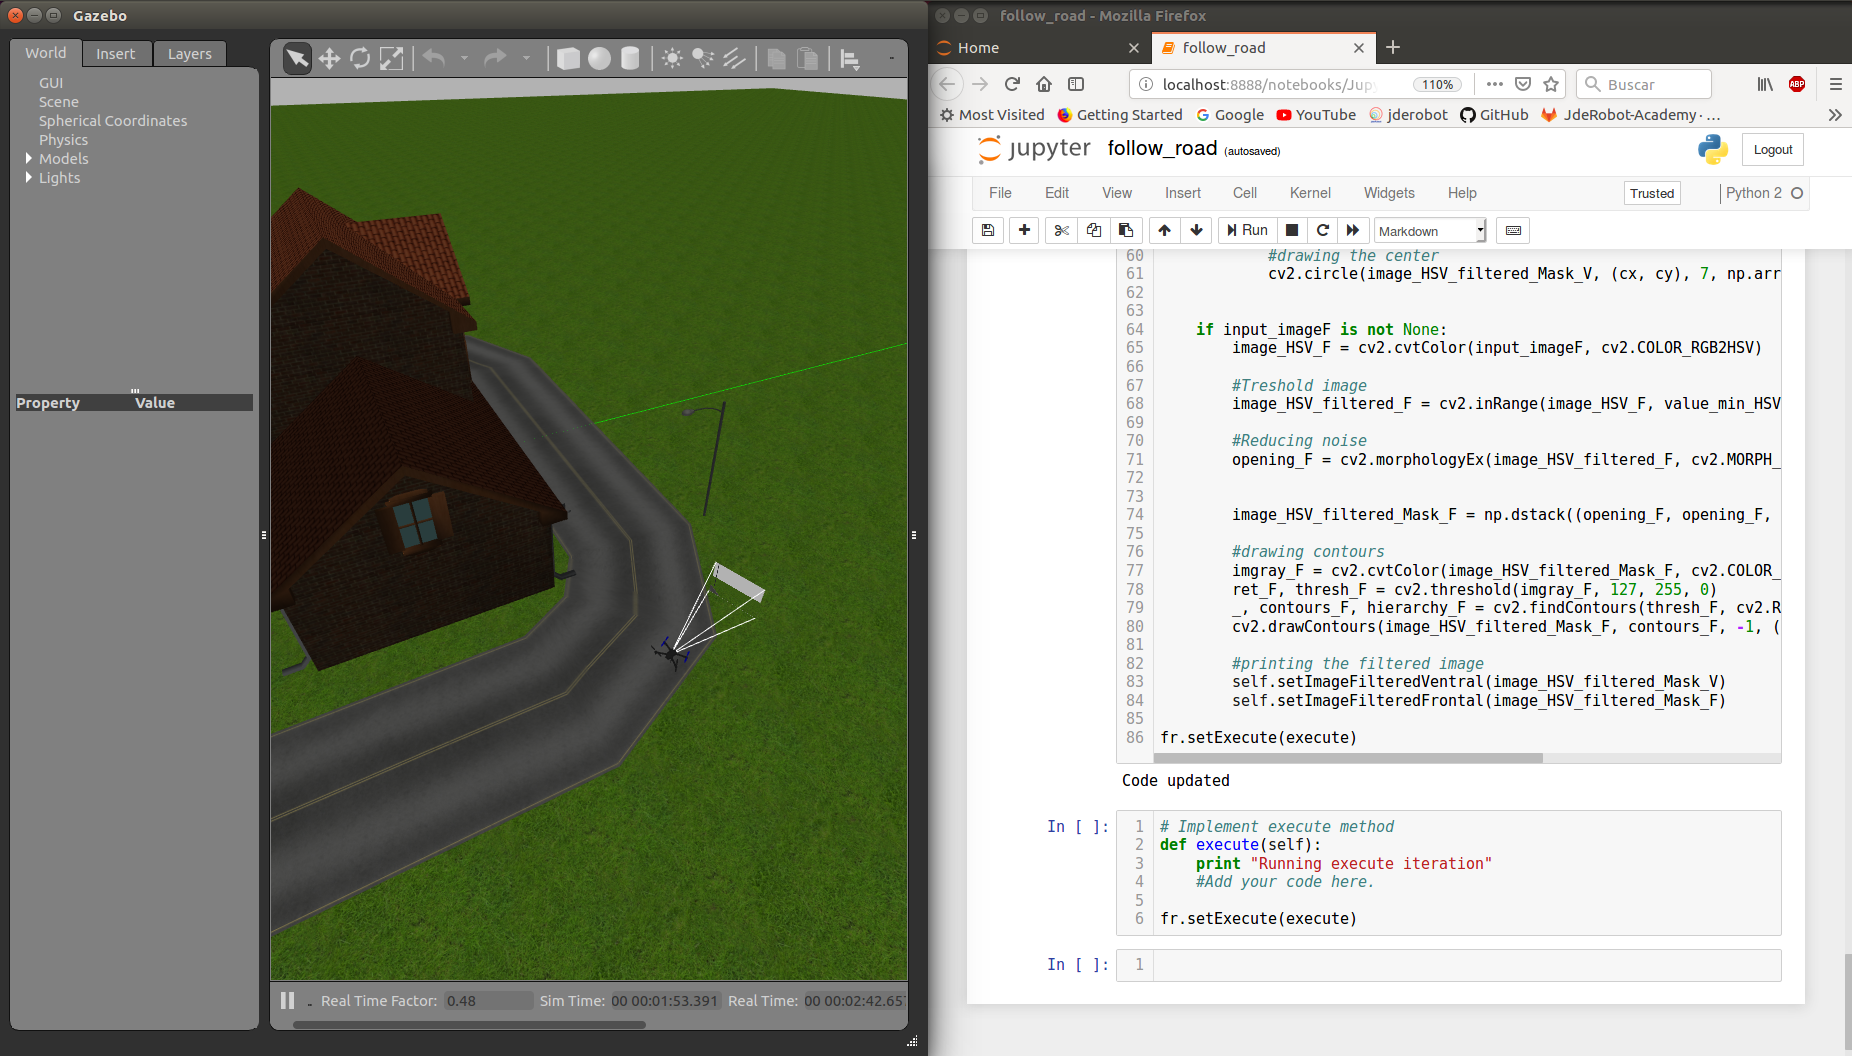
\includegraphics[width=0.7\textwidth]{figures/ejec_3_jup_fr.png}
		\caption{Ejecución del código del ejercicio Follow Road desde un navegador web (c)}
		\label{fig.ecjfr3}
		\end{center}
\end{figure}
